\documentclass{article}

%-------------------------%
% PREAMBUŁA --------------%
%-------------------------%
\usepackage[utf8]{inputenc}
\usepackage[OT4]{polski}
\usepackage{caption}
\usepackage{amsmath}
\usepackage{tikz}
\usepackage{subcaption}
\usepackage{tabularx}
\usepackage{caption}
\usepackage{array}
\usepackage{hyperref}
\usepackage{graphicx}
\usepackage{fancyhdr}
\usepackage[justification=centering]{caption}
\usepackage[margin=60pt]{geometry}



%\usepackage[T1]{fontenc}
%\usepackage{amsthm}
%\theoremstyle{plain}
%\usepackage{enumitem}
%\captionsetup[table]{skip=-4pt}
%\usepackage{tabulary}
%\usepackage{sidecap}
%\usepackage{gensymb}
%\usepackage{wrapfig}
%\usepackage{lastpage}
%\usepackage{gensymb}
%\usepackage{lipsum}
%\pagestyle{fancy}


\newlength{\RoundedBoxWidth}
\newsavebox{\GrayRoundedBox}
\newenvironment{GrayBox}[1][\dimexpr\textwidth-4.5ex]%
   {\setlength{\RoundedBoxWidth}{\dimexpr#1}
    \begin{lrbox}{\GrayRoundedBox}
       \begin{minipage}{\RoundedBoxWidth}}%
   {   \end{minipage}
    \end{lrbox}
    \begin{center}
    
\begin{tikzpicture}%
       \draw node[draw=black,fill=black!1,rounded corners,%
             inner sep=2ex,text width=\RoundedBoxWidth]%
             {\usebox{\GrayRoundedBox}};
    \end{tikzpicture}
    \end{center}}

%------- Typy kolumn do ustawiania szerokości ------- %
\newcolumntype{L}[1]{>{\raggedright\let\newline\\\arraybackslash\hspace{0pt}}m{#1}}
\newcolumntype{C}[1]{>{\centering\let\newline\\\arraybackslash\hspace{0pt}}m{#1}}
\newcolumntype{R}[1]{>{\raggedleft\let\newline\\\arraybackslash\hspace{0pt}}m{#1}}








\begin{document}

%-------------------------%
%Tabela nagłówkowa -------%
%-------------------------%

\begin{table}[h]
\begin{tabular}{|l|l|l|l|l|l|}
\hline
\begin{tabular}[c]{@{}l@{}}
Wydział:\\ WFiIS\end{tabular} &
\multicolumn{2}{l|}{\begin{tabular}[c]{@{}l@{}}
Imię i nazwisko:\\ 1. Axel Zuziak\\ 2. Marcin Węglarz \end{tabular}} 
& Rok \textbf{II}         
& Grupa \textbf{02}          
& Zespół \textbf{03}      \\ \hline
\textbf{\begin{tabular}[c]{@{}l@{}}
PRACOWNIA\\ FIZYCZNA \\ WFiIS AGH\end{tabular}} &
\multicolumn{4}{l|}{ Temat:\textbf{ Opracowanie danych pomiarowych} }                                                                                                                       & \multicolumn{1}{c|}{\begin{tabular}[c]{@{}c@{}}
Nr ćwiczenia\\ \textbf{00}
\end{tabular}} \\ \hline
\begin{tabular}[c]{@{}c@{}}
Data wykonania:\\ 04.03.2015
\end{tabular} &
\begin{tabular}[c]{@{}c@{}}
 Data oddania:\\ 18.03.2015
\end{tabular} &
\begin{tabular}[c]{@{}c@{}}
Zwrot do poprawy: \\ 
\end{tabular}                                 
& 
\begin{tabular}[c]{@{}c@{}}
Data oddania: \\ 
\end{tabular}&
\begin{tabular}[c]{@{}c@{}}
Data zaliczenia:\\
\end{tabular}& 
\begin{tabular}[c]{@{}c@{}}
OCENA:\\
\end{tabular}       
\\ & & & & & \\ \hline
\end{tabular}
\end{table}
%-----Koniec tabeli------

%-------------------------%
% ABSTRAKT ---------------%
%-------------------------%

\section{Abstrakt} 
	W ćwiczeniu wykonano prosty pomiar fizyczny 
	
%-------------------------%
% WSTĘP ------------------%
%-------------------------%

\section{Wstęp}
	W wahadle prostym poruszające się ciało jest punktem materialnym zawieszonym na nieważkiej, nierozciągliwej nici o długości $l$. Zakładając, że na ciało działa siła ciężkości skierowana w dół o wartości $g$, oraz oznaczając kąt wychylenia przez $\theta$ można zapisać równanie:
	\begin{equation}
		\frac{d^2\theta}{dt^2} = -\frac{g}{l}\sin{\theta}
		\label{wzor1}
	\end{equation}
	Przy małych wychyleniach kąta $\theta$ funkcję sinus można przybliżyć jej argumentem, co pozwala zapisać:
	\begin{equation}
		\frac{d^2\theta}{dt^2} +\omega^2\theta = 0
		\label{wzor2}
	\end{equation}
	Gdzie częstość kołowa drgań wynosi: $\omega = \frac{2\pi}{T}$. Czyli możemy wyznaczyć zależność okresu drgań wahadła:
	\begin{equation}
		T = 2\pi\sqrt{\frac{l}{g}}
		\label{wzor3}
	\end{equation}
	
	%-----------------------------------------%
% Aparatura i wykonanie ćwiczenia --------%
%-----------------------------------------%
\section{Aparatura i wykonanie ćwiczenia}
	W ćwiczeniu wykonano dwie serie pomiarów:
	\begin{enumerate}%Spróbuj użyć innego słowa niż linijka :)
		\item \textbf{Pomiary dla ustalonej długości wahadła.}\\
			Zmierzono długość wahadła za pomocą linijki. Wprowadzono wahadło w ruch drgający o bardzo małej amplitudzie rzędu kilku stopni. Zmierzono czas $k= XXX$ okresów. Pomiar powtórzono dziesięciokrotnie. (zmieniając lub nie zmieniając liczy okresów). Wyniki przedstawiono w tabeli (1).
		\item \textbf{Pomiary zależności okresu drgań od długości wahadła.}\\
			Wykonano LICZBA pojedynczych pomiarów okresu, zmieniając długość wahadła w zakresie (ZAKRES).
	\end{enumerate}
	W obu pomiarach użyto następującej aparatury:
	\begin{itemize} %% Uzupełnij Twoimi danymi
		\item \textbf{Stoper} marki HTC o niepewności: $\Delta t = 0,1s$
		\item \textbf{Linijka} o najmniejszej podziałce $\Delta d = 0,1$ cm.
		\item \textbf{Sześciokątna nakrętka} - w przybliżeniu punktowa masa.
		\item \textbf{Sznurek} - w przybliżeniu nieważka nić. % napisz jaki (jaki?jak regulowana długość? kilka sznurków?)
	\end{itemize}
	
%--------------------------%
% Wyniki pomiarów ---------%
%--------------------------%
\newpage

\section{Wyniki pomiarów}

%-------------TABELA 1------------------%
	\setlength\extrarowheight{2pt} % zwiększa wysokość komórek o 2pt
\textbf{Długość wahadła:} $l = 19,0 \pm 0,1$ cm. %

	\begin{table}[h]
		\centering
		\caption{Wyniki pomiarów okresu drgań przy ustalonej długości wahadła}
		\begin{tabular}{|C{1cm}|C{1.8cm}|C{2.5cm}|C{2.5cm}|} % Tak się używa tych kolumn
			\hline
			L.P & Liczba okresów $k$ & Czas $t[s]$ dla $k$ okresów & Okres $T_i = t/k[s]$ \\ \hline
			1& 40 & 34,1 &	0,8525 \\ \hline
			2& 40 & 35,1 &	0,8775 \\ \hline
			3& 40 & 35,1 &	0,8775 \\ \hline
			4& 40 & 35,1 &	0,8775 \\ \hline
			5& 40 & 35,0 &	0,8750 \\ \hline
			6& 40 & 35,0 &	0,8750 \\ \hline
			7& 40 & 35,0 &	0,8750 \\ \hline
			8& 40 & 35,1 &	0,8775 \\ \hline
			9& 40 & 34,9 &	0,8725 \\ \hline
			10&	40 & 35,0 &	0,8750 \\ \hline
		\end{tabular}
		\label{tabela1}
	\end{table}
	
%-------------TABELA 2------------------%
	\setlength\extrarowheight{2pt}
	\begin{table}[h]
		\centering
		\caption{Wyniki pomiarów zależności okresu drgań od długości wahadła}
		\begin{tabular}{|C{1cm}|C{1.8cm}|C{1.8cm}|C{2.2cm}|C{2cm}|C{2cm}|}\hline
			L.P & $l$ [mm] & k & $t$ [s] & $T_i$ [s] & $T_i^2$ [$\text{s}^2$] \\ \hline
			1 & 110 & 20 & 13,3 & 0,665 & 0,44222 \\\hline 			
			2 & 125 & 20 & 14,2 & 0,71 & 0,5041 \\ \hline
			3 & 130 & 20 & 14,3 & 0,715 & 0,511225 \\ \hline
			4 & 135 & 20 & 14,6 & 0,73 & 0,5329 \\ \hline
			5 & 145 & 20 & 15,2 & 0,76 & 0,5776 \\ \hline
			6 & 150 & 20 & 15,4 & 0,77 & 0,5929 \\ \hline
			7 & 155 & 20 & 15,7 & 0,785 & 0,616225 \\ \hline
			8 & 160 & 20 & 15,9 & 0,795 & 0,632025 \\ \hline
			9 & 165 & 20 & 16,1 & 0,805 & 0,648025 \\ \hline
			10 & 170 & 20 & 16,4 & 0,82 & 0,6724 \\ \hline
			11 & 175 & 20 & 16,6 & 0,83 & 0,6889 \\ \hline
			12 & 180 & 20 & 16,8 & 0,84 & 0,7056 \\ \hline
			13 & 185 & 20 & 17,1 & 0,855 & 0,731025 \\ \hline
			14 & 190 & 20 & 17,5 & 0,875 & 0,765625 \\ \hline
			15 & 195 & 20 & 17,7 & 0,885 & 0,783225 \\ \hline		
		\end{tabular}
		\label{tabela2}
	\end{table}
	
%--------------------------%
% Wyniki obliczeń ---------%
%--------------------------%

\section{Wyniki obliczeń}
 \begin{itemize}
	\item Analizując wyniki pomiarów z dalszych obliczeń wykluczono pozycje $1$ z tabeli (\ref{tabela1}).
		
	\item Następnie wyliczono niepewność typu A wyznaczenia okresu drgań wahadła jako estymator odchylenia standardowego średniej oraz wartość
	średnią liczoną jako średnia arytmetyczna wyników.\\\\
	 $\overline{T} = 0,8735$ s.\\ % nie wiem jak to ładnie ułożyć na stronie
	 $u_A(T) = 0,0024$ s
	
	%	\begin{equation*}
	%		u_A(T) = \sqrt{ \frac{(1,45 - 1,43)^2 + (1,41 - 1,43)^2 + \dots + (1,42 - 1,43)^2 }{ 10(10-1) } } = 0,0001234 \; \text{s}
	%	\end{equation*}

	\item Niewność pomiaru długości wahadła określono jako niepewność typu B i przyjęto wartość działki elementarnej: \\\\ % podziałka złe słowo
		$u_B(l) = 0,1$ cm.\\ % nie wiem jak to ładnie ułożyć na stronie
		
	\item W celu wyznaczenia przyśpieszenia ziemskiego przekształcono wzór (\ref{wzor3}) do postaci:
		\begin{equation}
			g = \frac{4\pi^2\cdot l}{T^2}
		\end{equation}
		Po podstawieniu:\\\\
		\[ g = 9,831 \frac{m}{s^2} \]\\
		 
	%	\begin{equation*}
	%		g = \frac{3\cdot 3,14^2 \cdot 0,02}{1,43^2} = 9,822 \; \frac{\text{m}}{\text{s}^2}
	%	\end{equation*}
		
	\item Korzystając z prawa przenoszenia niepewności obliczono niepewność złożoną $u_c(g)$ wyznaczenia wartości przyśpieszenia ziemskiego.
		
		\begin{equation*}
			u_c(g) = \sqrt{ \left[ \frac{4\pi^2}{T^2}\cdot u(l) \right]^2 + \left[ -\frac{8\pi^2 l}{T^3} \cdot u(T) \right]^2 }
			 = 	0,075 \frac{m}{s^2}
		\end{equation*}\\
	Oba człony składające się na niepewność $g$ mają porównywalne wartości.\\
	
	
	
	\item Kolejno narysowano wykres okresu od długości wahadła $T(l)$ oraz naniesiono na niego krzywą \\
	$f(x)=2\pi\sqrt{\frac{x}{g}}$\\
	
	\begin{figure}[ht]
		\centering
		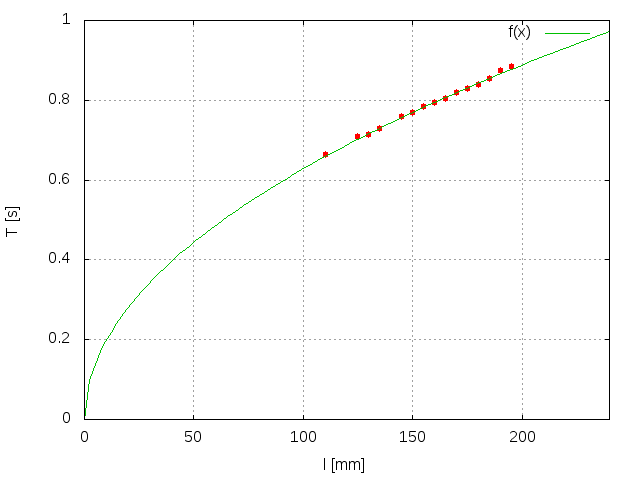
\includegraphics[width=0.7\textwidth]{wykres_T/wykres1.png}
		\caption{Wykres zależności okresu wahadła od jego długości.}
		\label{wykres1}
	\end{figure}
	
	
	
	\item Chcąc wyznaczyć wartość przyspieszenia $g$ graficznie, narysowano wykres funkcji, 
	gdzie na osi $y$ odłożono wartości $T^2$ a na osi $x$ długość wahadła $l$. Następnie korzystając z funkcji gnuplota dopasowano prostą $y=ax$ do punktów pomiarowych, gdzie wyznaczony współczynnik $a$: \\
	\[a = 3,968 \pm 0,010
	\]
	
	\begin{figure}[ht]
		\centering
		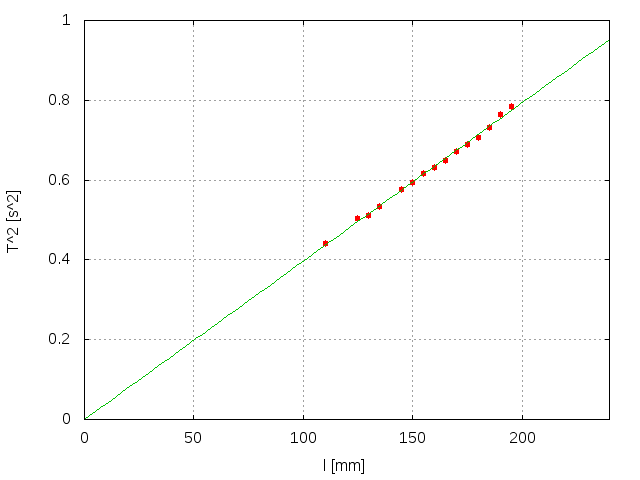
\includegraphics[width=0.7\textwidth]{wykres_T2/wykres2.png}
		\caption{Wykres zależności kwadratu okresu wahadła od jego długości.}
		\label{wykres2}
	\end{figure}
	
	Przekształcając wzór (\ref{wzor3}) poprzez podniesienie go do kwadratu i przyrównując go do funkcji liniowej $y=ax$ otrzymano wzór na $a$:\\
	\[a=\frac{4\pi^2}{g}
	\]\\
	W kolejnym kroku wyliczono $g$ z powyższego wzoru oraz $u(g)$ przy pomocy wartości $u(a)$ z prawa przenoszenia niepewności:\\
	\[u(g) = \frac{4\pi^2}{a^2}u(a) = 0,025 \frac{m}{s^2}
	\]\\
	Po podstawieniu:\\
	\[g = 9,949 \pm 0,025 \frac{m}{s^2}
	\]
	

  \end{itemize}

	
	


%\begin{GrayBox}
 %   \begin{centering}
  %       $\eta_0 = 1,455\;\;$Pa$\cdot$s.
   %     \vspace{3pt}
    %    \\$U(\eta) = 0,1\;\;$Pa$\cdot$s.
     %   \vspace{3pt}

   %     Różnica $|\eta - \eta_0| = 0,975\;\;$Pa$\cdot$s.

    %\end{centering}

%\end{GrayBox}


%%%%%%%%%%%% BIBLIOGRAFIA %%%%%%%%%%%%

\begin{thebibliography}{9}
 
\bibitem{lamport94}
  Robert Resnick, David Halliday
  \emph{Fizyka Tom 1}.
    Wydawnictwo Naukowe PWN, Warszawa,
  Wydanie piętnaste,
  2001.


 \bibitem{lamport94}
 Henryk Szydłowski,
 \emph{Pracownia fizyczna}, Wydawnictwo Naukowe PWN, Warszawa, Wydanie siódme, 1994.
  \bibitem{lamport94}
  Z. Stęgowski,
  \emph{Zeszyt A1 do ćwiczeń laboratoryjnych z fizyki}, Kraków, Akademia Górniczo Hutnicza im. Stanisława Staszica, dostępny na stronie:\\
  \url{http://www.fis.agh.edu.pl/~pracownia_fizyczna/cwiczenia/01_opis.pdf}
 \bibitem{lamport94}
 Jacek Tarasiuk,
 \emph{Wykłady, Statystyka Inżynierska} [on-line], Kraków, Akademia Górniczo Hutnicza im. Stanisława Staszica, dostępny na stronie:\\
  \url{http://home.agh.edu.pl/~tarasiuk/dydaktyka/index.php/statystykainzynierska}
\bibitem{lamport94}
  Małgorzata Nowina-Konopka, Andrzej Zięba,
  \emph{Ćwiczenie 13. Współczynnik lepkości}, Kraków, Akademia Górniczo Hutnicza im. Stanisława Staszica, dostępny na stronie:\\
  \url{http://www.ftj.agh.edu.pl/zdf/zeszyt/3_13n.pdf}


\end{thebibliography}
\vspace{2cm}



\end{document}











\end{document}
